\documentclass{parasim}
\usepackage{graphicx}

\title{Zpráva za období červen až červenec 2012}
\begin{document}
\section{Druhá etapa}

\subsection{Popis}

Ve druhé etapě probíhající od června do července 2012 jsme se zabývali tvorbou testů 
a dokumentace, hledáním vhodných modelů pro analýzu, profilováním a drobnými úpravami
nástroje.

Ve zkratce lze tedy říci, že bylo vyřešeno následující:

\begin{itemize}
    \item   dokumentace k jednotlivým rozšířením výpočtu a vizualizace,
    \item   refaktoring jádra aplikace potřebný k dalšímu rozšířování,
    \item   rozšíření pro měření výkonu aplikace,
    \item   testy a testovací modely,
    \item   měření výkonu jednotlivých částí aplikace.
\end{itemize}

Vydaná verze je k dispozici na stránkách našeho projektu\footnote{\url{https://github.com/sybila/parasim/zipball/1.0.0.M2}},
kde najdete též seznam vyřešených úkolů\footnote{\url{https://github.com/sybila/parasim/issues?milestone=4&page=1&state=closed}}.

\subsection{Výsledky měření}

Nástroj byl postupně spouštěn nad třemi dostupnými testovacími modely. Cílem bylo
změřit podíl jednotlivých částí algoritmu na celkovém čase. Konfigurace testovacího
stroje byla následující:

\medskip

\begin{center}
\framebox[\textwidth]{\parbox{0.9\textwidth}{\small
Java(TM) SE Runtime Environment (build 1.7.0\_04-b20), Java HotSpot(TM) 64-Bit Server VM (build 23.0-b21, mixed mode),
Linux version 2.6.43.8-1.fc15.x86\_64, Intel(R) Core(TM) i7-2620M CPU @ 2.70GHz (4 jádra), 4 GB paměti
}}
\end{center}

\subsubsection{Experiment \texttt{test-1}}

\begin{figure}[H]
    \centering
    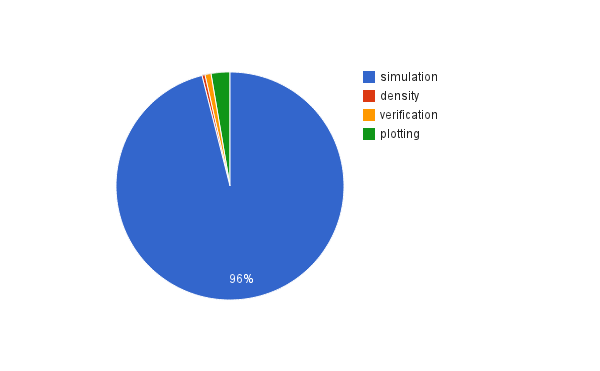
\includegraphics[width=0.75\textwidth]{1.0.0.M2/test-1.png}
\end{figure}

\subsubsection{Experiment \texttt{test-2}}

\begin{figure}[H]
    \centering
    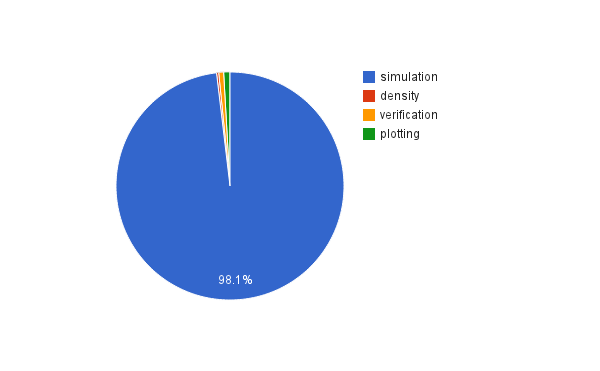
\includegraphics[width=0.75\textwidth]{1.0.0.M2/test-2.png}
\end{figure}

\subsubsection{Experiment \texttt{test-3}}

\begin{figure}[H]
    \centering
    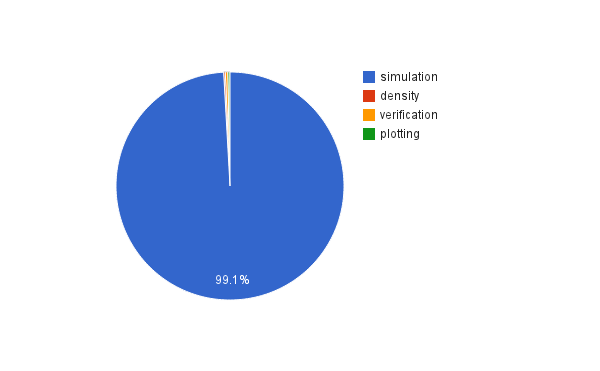
\includegraphics[width=0.75\textwidth]{1.0.0.M2/test-3.png}
\end{figure}

\end{document}
